\chapter{Estado da Arte}
% OU \chapter{Trabalhos Relacionados}
% OU \chapter{Engenharia de Software}
% OU \chapter{Tecnologias e Ferramentas Utilizadas}
\label{chap:estado-da-arte}

\section{Introdução}
\label{chap2:sec:intro}
Cada capítulo \underline{intermédio} deve começar com uma breve introdução onde é explicado com um pouco mais de detalhe qual é o tema deste capítulo, e como é que se encontra organizado (i.e., o que é que cada secção seguinte discute). 



-----

Python

\section{Estado atual do reconhecimento de Objetos}
\label{chap2:sec:estado}





\section{Funcionamento do Reconhecimento de Objetos}
\label{chap2:sec:funcionamento}




\section{Algoritmos Estudados}
\label{chap2:sec:algoritmos}


ver relatório dado pelo professor




\section{Algortimos de Deteção de Objetos}
\label{chap2:subsec:algoritmosdetecao}

\subsection{color thresholding + contour extraction}

Cor limiar e extração de contorno

Métodos basicos de cor limiar 

\subsection{Haar cascades}

\subsection{HOG + Linear SVM}

\subsection{SSDs}

\subsection{Faster R-CNNs}

\subsection{Yolo}
\paragraph{}
\textit{Yolo (You Only Look Once)} é um algortimo de deteção de objetos que aceita um feed de video em tempo real.
No Yolo, com uma unica CNN ??? ??? simultanemente prevemos multiplas caixas delimitadoras e probabilidades de classes para essa caixa. O Yolo treina em imagens completas e otimiza diretamente o desempenho da deteção. Este modelo afirma ter um numero de beneficios sobre outros métodos de deteção de objetos, como:
\newline - YOLO encontra todos os objetos em uma imagem simultanemente.
\newline - Usa uma unica rede convulcional para toda a imagem.
\newline - Usa carateristicas da imagem inteira para prever cada caixa.delimitadora. Tambem preve todas as caixas delimitadoras de todas as classes para uma imagem simultanemanete. Prevê as caixas delimitadoras e as probabilidades de classe para essas caixas.
\newline - YOLO vê a imagem inteira durante o treino e tempo de teste, portanto codifica implicitamente informações contextuais sobre classes tal como a sua aparencia.
\newline - YOLO aprende representações generalizadas de objetos para que quando treinado em imagens naturais e testado em obras de arte, o algoritmo supera outros modelos de deteção.

\paragraph{Trabalho do YOLO}
\paragraph{}

- YOLO pega em uma imagem e divide-a em uma rede SxS. Cada célula prevê apenas um objeto.
- A clissificação e localização da imagem são aplicados em cada célula.
- Se o centro de um objeto fica em uma célula, essa célula é responsavel por detetar esse objeto.
- Cada célula da rede prevê B caixas delimitadoras com classificações de confiança para essas caixas.

1. Caixas de confiança refletem o quão confiante o modelo está sobre a caixa conter o objeto e quão preciso ele pensa a caixa ser o que ele pensa. Se o objeto não existir, então a classificação de confiança será zero. 
\newline
A previsão de confiança reprensenta a IOU entre a caixa de previsão e qualquer caixa de verdade do solo.
Pr(Object) * IOU verdade previsão - interseção de união (IOU) entre a caixa prevista e o verdadeiro solo.







The output of the algorithm is a list of bounding box, in format [class, x, y, w, h, confidence]. The class is an id related to a number in a txt file (0 for car , 1 for pedestrian, …). x, y, w and h represent the parameters of the bounding box. x and y are the coordinates of the center while w and h are its size (width and height). The confidence is a number expressed in %.

\subsection{Tensorflow}
\label{chap2:subsec:tensorflow}

Tensorflow Lite


\subsection{OpenCV}
\label{chap2:subsec:opencv}
\paragraph{}

Opencv é uma biblioteca \textit{open source} criada em 2000 pela Intel e com Licença BSD Intel para a sua Distribuição. Utilizada para o desenvolvimento de aplicações na área de computação visual, seja para o uso acadêmico ou comercial. Possui módulos para processamento de imagens, estrutura de dados, àlgebra linear, bem como uma interface gráfica para usuário e mais de 350 algoritmos de visão computacional, como filtros de imagem, calibração de câmera, reconhecimento de objetos, análise estrutural e outros.


\section{Algortimos de Rastreamento de Objetos}
\label{chap2:subsec:algoritmosrastreamento}



\subsection{Centroid tracking}
\label{chap2:subsec:centroidtraking}



\paragraph{}
\textit{Centroid traking} é um algoritmo presente na biblioteca OpenCV, que depende da distância euclidiana\footnote{Dintância entre dois pontos} entre centróides de objetos (ex. objetos que o rastreador de centróide já viu antes) e novos centróides de objetos entre quadros subsequentes em um video.

O algoritmo de rastreamento de centróides é um processo de multiplas etapas:

\paragraph{1- Aceitar as coordenadas da caixa delimitadora do objeto e calcular os centróides}
\paragraph{}
Este algoritmo assume que estamos a passar um conjunto delimitador de coordenadas 2D de cada objeto detectado em \textit{every single frame} (cada frame de video).
\newline
Estas caixas delimitadoras podem ser produzidas por qualquer tipo de detetor de objetos que mais gostemos (temos em este capitulo alguns algoritmos de delimitadores explicados).
\newline
Depois de obtermos as coordenadas das caixas delimitadoras, devemos determinar o centróide, ou simplesmente, o centro da caixa.
\newline
Visto que este é o conjunto inicial de caixas, devemos lhes atribuir IDs unicos.
\begin{center}
  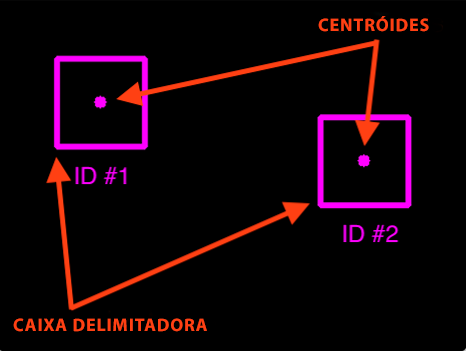
\includegraphics[scale=0.5]{simple_object_tracking_step1.png}
  \label{img:centroid_traking1}  
\end{center}

\paragraph{2- Calcular distância euclediana entre novas caixas delimitadoras e objetos existentes}
\paragraph{}
Para cada subsequente frame do nosso video, aplicamos a etapa 1 de calcular os centróides de cada objeto. Porem aqui, invês de atribuir um ID unico a cada objeto detectado (que iria contrariar o sentido de rastrear um objeto), precisamos determinar primeiro se podemos acociar novos centróides de objetos (pontos amarelos) a aos centróides antigos (pontos roxos). Para este processo, nós calculamos a distância euclediana entre cada par de objetos existente e novos objetos.
\newline
Mas como vamos usar as distâncias Eucledianas entre estes pontos para combiná-los e associá-los? 

\begin{center}
  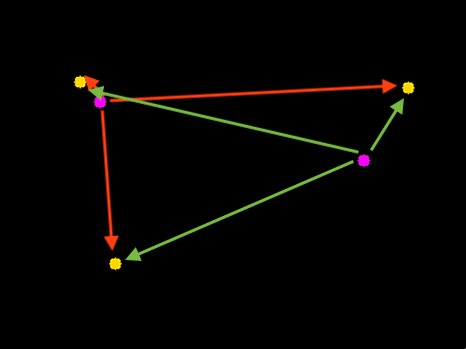
\includegraphics[scale=0.5]{simple_object_tracking_step2.png}
  \label{img:centroid_traking2}  
\end{center}

\paragraph{3- Atualizar coordenadas para objetos existentes}
\paragraph{}
A supozição primária do algoritmo de rastreamento de centroides de objetos é de que o objeto irá se potencialemente mover entre frames subsequentes, porem a distância entre centróides será menor que outras distâncias entre objetos.
\newline
Portanto, se escolhermos associar centróides com a menor distância entre frames subsequentes, podes construir o nosso rastreador de objetos.
\newline
Mas e se surgir um novo objeto? 

\begin{center}
  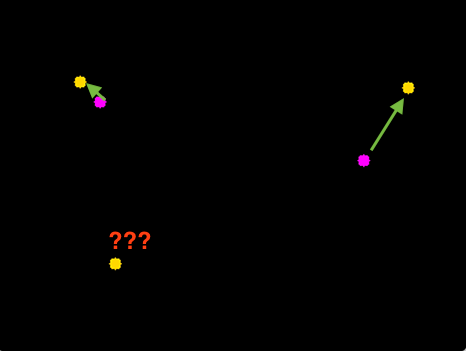
\includegraphics[scale=0.5]{simple_object_tracking_step3.png}
  \label{img:centroid_traking3}  
\end{center}


\paragraph{4- Registar novos objetos}
\paragraph{}
No caso de obtermos mais objetos detetados do que objetos a ser rastreados, precisamos registar o novo objeto. Registar o novo objeto na lista de objetos a ser rastreados significa que: 
\newline - Atribuimos um novo ID
\newline - Guardamos o centróide da caixa delimitadora para esse objeto
\newline
Podemos ir até a etapa 2 e repetir o processo de etapas em cada frame de video.

\begin{center}
  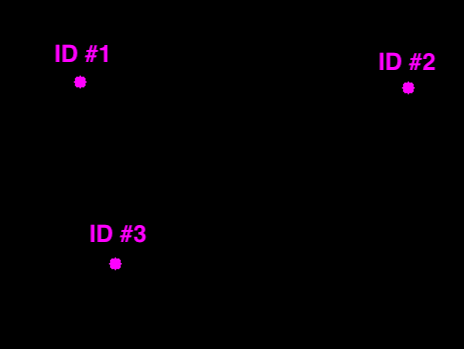
\includegraphics[scale=0.5]{simple_object_tracking_step4.png}
  \label{img:centroid_traking4}  
\end{center}



ref: 
https://www.pyimagesearch.com/2018/07/23/simple-object-tracking-with-opencv/


\subsection{Hungarian Algorithm (Kuhn-Munkres)}
\label{chap2:subsec:hungarian}

A Hungarian algorithm can tell if an object in current frame is the same as the one in previous frame. It will be used for association and id attribution

https://towardsdatascience.com/computer-vision-for-tracking-8220759eee85

\subsection{Kalman Filter}
\label{chap2:subsec:kalman}


A Kalman Filter is an algorithm that can predict future positions based on current position. It can also estimate current position better than what the sensor is telling us. It will be used to have better association.

https://towardsdatascience.com/computer-vision-for-tracking-8220759eee85




































\section{Citações e Referências Cruzadas -- [RETIRAR DA VERSÃO FINAL]}
\label{chap2:sec:citacoes}

Para se referenciarem outras secções, usar \texttt{\textbackslash{}ref\{label\}}, e.g., para citar a secção da Introdução deste capítulo, usar \texttt{\textbackslash{}ref\{chap2:sec:intro\}}. O resultado é: a secção~\ref{chap2:sec:intro} contém a introdução deste capítulo.

Para se citarem fontes bibliográficas, \underline{colocar a entrada certa} no ficheiro \texttt{bibiografia.bib} e usar o comando \texttt{\textbackslash{}cite\{label-da-referencia\}}, ligando o comando com a palavra que o antecede com um til. Por exemplo, para citar a referência eletrónica \emph{The Not So Short Introduction to \LaTeX{}}~\cite{short}, deve incluir-se o trecho seguinte no ficheiro \texttt{bibiografia.bib} e usar \texttt{\textbackslash{}cite\{\underline{short}\}} para a citação (citação incluída nesta mesma frase):
%
\begin{verbatim}
@MISC{short,
  author = {Tobias Oetiker and Hubert Partl and Irene Hyna and Elisabeth Schlegl},
  title  = "{The Not So Short Introduction to \LaTeX{}}",
  year   = 2018,
  note   = {[Online] \url{https://tobi.oetiker.ch/lshort/lshort.pdf}. 
            Último acesso a 12 de Março de 2019}
}
\end{verbatim}


\section{Secções Intermédias}
\label{chap2:sec:...}

\section{Conclusões}
\label{chap2:sec:concs}

Cada capítulo \underline{intermédio} deve referir o que demais importante se conclui desta parte do trabalho, de modo a fornecer a motivação para o capítulo ou passos seguintes.